%-*- coding: UTF-8 -*-
% body.tex
% 这个文件是文章的主要内容,包括从introduction到reference的全部内容。
\section{Introduction}

\subsection{Background}
With the increase in terrorist attacks in recent years, the world is committed to preventing terrorist attacks. However, god's way is higher than man's. The number of deaths due to terrorist attacks is still increasing in the worldwide. As a result, reviews of many popular attractions should be put on the agenda.The Louvre is the world's largest and most visited art museum , any exhibit in it can be said to be the treasure of the world. Its fame also makes it easier to be the target of attack, so it becomes a hot discussion topic to provide a reasonable emergency evacuation plan for Louvre.
 
%随着近几年恐怖袭击事件的增加,全世界都在致力于如何预防恐怖袭击的发生。God's way is higher than man's.由于恐怖袭击的致死人数依然在增加。因此,对于许多热门景点的审查被提上了日程。卢浮宫是世界上参观人数最多的也是最大的博物馆,里面的随便一件展品都可以说是世界的珍宝。他的著名也使得它更容易成为被袭击的目标,那么为它在紧急情况下提供一个合理的疏散方案就变成了一个热门的讨论话题
\subsection{Restatement}
%当我们考虑卢浮宫的疏散问题,我们需要考虑不同游客疏散的时间和路线安排。为了
When we consider the evacuation of the Louvre, we need to consider the time and route of evacuation of different tourists. In order to evacuate visitors from the museum, while also allowing emergency personnel to enter the building as quickly as possible, we are required to answer the following questions.
\begin{itemize}
    \item Develop an emergency evacuation model which should evacuate the visitors from the museum, while also allowing emergency personnel to enter the building quickly.
    \item The model should be an adaptable model.
    \item Consider the number of visitors and the diversity  of visitors when implement our model in Louvre
    \item Consider carefully when and how any additional exits might be utilized.
    \item Propose some policy and procedural recommendations for emergency management of Louvre and implement our model for other large,crowd structures.
    \item Think how technology, such as apps like \emph{Affluences}, or others could be used to facilitate our evacuation plan.
    
\end{itemize}

\subsection{Literature Review}
%目前,法国的恐怖袭击事件日益增加,安全形势日益严峻。而卢浮宫是世界访客人数最多的博物馆。所以很有必要对人员疏散问题提起高度注意。
At present, the terrorist attacks in France are increasing and the security situation is becoming increasingly serious. The Louvre is the most visited museum in the world. Therefore, it is necessary to pay great attention to the evacuation of personnel.
%目前,已经有很多文献对人员疏散问题进行研究,方法较为成熟。甚至已经有专业的软件可以对人员疏散问题进行模拟仿真,如Pathfinder和Anylogic。
At present, there is much literature on the issue of evacuation of people, and the method is relatively mature. There are even professional software that can simulate the evacuation of personnel, such as $Pathfinder$ and $Anylogic$.
%对于人员的疏散问题,广泛采用的方法是利用元胞自动机。如 和 。事实上,元胞自动机建立的模型有很多不足,例如正方形方格的划分使得斜着走并不可能,以至于移动距离增大了很多。

For the evacuation of personnel, the widely used method is to use a cellular automaton. Such as \cite{yang2005simulation}and\cite{wolf2004lattice}. In fact, the model built by the cellular automaton has many shortcomings. For example, the grid division makes it impossible to slant, so that the moving distance increases a lot.
%还有一些模型利用BIM,也能够给问题提供一个较为合理的思路,如 和 。
There are also some models that use BIM and dynamic planning to provide a more reasonable idea of the problem, such as \cite{lin2008use}and \cite{wang2014bim}.
%一些人另辟蹊径,从火灾中人的行为和心理进行分析,也能提出一些有效、有价值的措施帮助我们解决人员疏散的问题,如 和 。
Some people have taken a different approach and analyzed the behavior and psychology of people in the fire. They can also propose effective and valuable measures to help us solve the problem of evacuation, such as \cite{jin2002visibility}.
%还有一些文献直接对人的行为进行模拟,做出了一些通用的可用于人群的模型,也解决了人群疏散问题。
There are also some literature that directly simulate human behavior. They have made some common models that can be used for people and solved the problem of crowd evacuation, such as \cite{pelechano2007controlling} and \cite{thalmann2007crowd}.

\subsection{Our Work}
The  overall objectives of our model is listed as follows:

\begin{enumerate}
    \item Design a pragmatic function for the movement of people.Meanwhile,set a reasonable objective function to accurately calculate the total minimum time for people on each floor to complete the evacuation and thereby divide the area to several safety response zone that each exit can radiate
    \item By abstracting the topographic map of each floor into an undirected network, we plan the best way for people on this floor to get to the designated exit.
    \item  Inter-floor Sorting Model is established to visually describe the PF after superimposed on two floors
    \item In order to make our model more convincing and adaptable, we have also made a number of recommendations for managers of the place where emergency occurs, which involve all aspects of an evacuation.
    \item We validate our models and discuss how the Louvre would implement it.
\end{enumerate}

\begin{figure}[H]
    \centering
    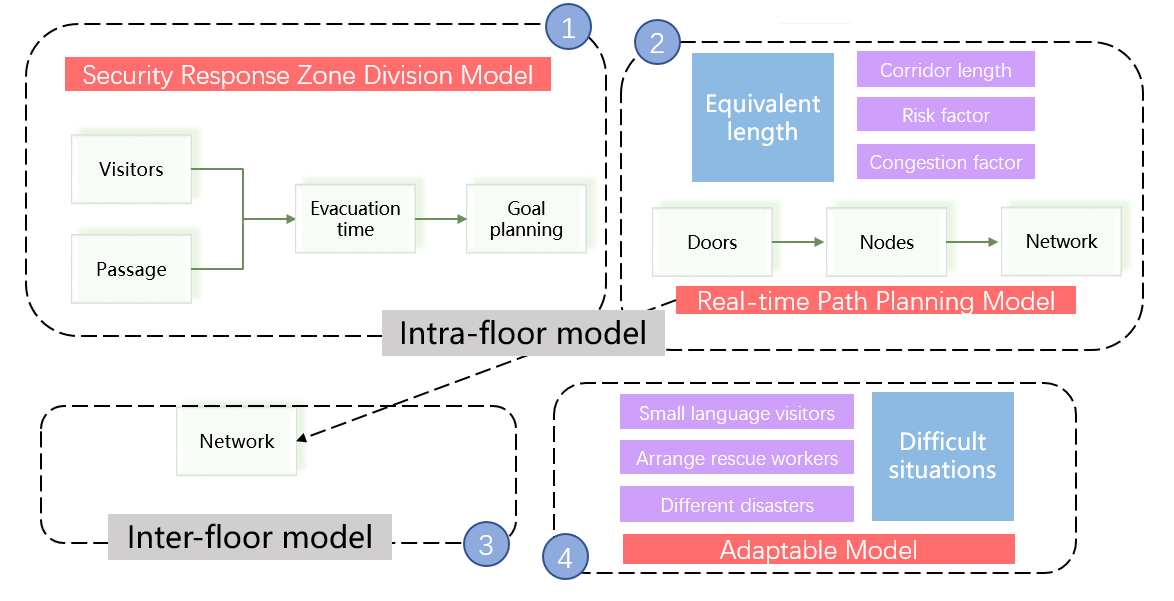
\includegraphics[scale=0.7]{all.png}
    \caption{Our Work}
    \label{all}
\end{figure}

\section{Preparation of the Models}
\subsection{Assumptions}

\begin{itemize}
    \item \textbf{We assume that the official evacuation instructions have a strong guiding effect on tourists.} 
    
    \textbf{Justification:} from a psychological point of view, when a security incident occurs, people are affected by panic and fear, and at this time, authoritative guidance is extremely needed.
    \item \textbf{We assume that the elevator is not used by normal people during emergency evacuation.}
    
    \textbf{Justification:} based on case studies of security incidents and inquiries from professionals, the use of elevators increases safety hazards when security incidents occur

    \item \textbf{We assume that everyone on the same floor knows an emergency at the same time.}
    \item \textbf{We assume that staircase can be used as escape routes in any case .}
    
     

\end{itemize}
\subsection{Terminology}
\paragraph{PF:}It is defined as the people flow, which is the number of people who pass the effective section per unit time.
\paragraph{SRZ:}It is defined as the safety response zone, which divides a floor into different evacuation areas.
\subsection{Notations}
The primary notations used in this paper are listed in \textbf{Table \ref{Ntt}}.
\begin{table}[h]
    \begin{center}
        \caption{Notations}
        \begin{tabular}{cl}
            \toprule
            \multicolumn{1}{m{3cm}}{\centering Symbol}
            &\multicolumn{1}{m{8cm}}
              {\centering Definition}\\
            \midrule
            $F$&The export capacity\\
            $T_e$&The time for evacuation\\
            $\omega_{ij}$ &The equivalent coefficient in the node\\
            $k$ &The hazard index to evaluate the danger degree\\
            $\Delta$ &The acceptable group number\\
            \bottomrule
        \end{tabular}\label{Ntt}
    \end{center}
\end{table}



\section{Security Response Zone Division Model}

\subsection{Model Overview and Analysis}
When security incidents occur in large public places such as museums, it is highly prone to tourists' conflicts, trampling, and casualties due to intensive tourists and disordered orders. Therefore, when we establish an emergency evacuation plan for the Louvre, we must first divide the Security response zone (SRZ)for each of its floors. The division of the SRZ is set according to the exit location and the regional tourist density. When a security incident occurs, the visitor security personnel and staff guide the tourists to evacuate as soon as possible in the SRZ, and avoid cross-regional evacuation activities to reduce the occurrence of tourist conflicts, improve the efficiency of evacuation, and ensure the safety of tourists.

%当博物馆等大型公共场所发生安全事件时,由于游客密集、秩序混乱等问题,极易导致游客冲突、踩踏、伤亡事件。因此,我们在为卢浮宫建立应急疏散方案时,首先要对它的每一层划分安全响应区。安全响应区的划分是依照出口位置和区域游客密度来设定的。当安全事件时,游客安保人员和工作人员引导游客在安全响应区内尽快疏散,并避免跨区域疏散行为,以减少游客冲突事件的发生,提高疏散的效率,保证游客的安全。
\subsection{Model Construction}
\subsubsection{Security Response Zone Model}

In order to avoid the occurrence of tourist conflicts as much as possible, we establish our zoning model according to the two principles of safety and efficiency. The number of the SRZs is equivalent to the number of exports. We use the shortest evacuation time as the objective function to build a programming model.
%我们为了尽可能的避免游客冲突事故的发生,我们依照安全和高效两项原则建立我们的区域划分模型。因此我们决定划分出与出口数目相当的安全响应区。我们以疏散时间最短作为目标函数建立线性规划模型。

Considering the actual situation, we use a combination of experience zoning and real-time adjustment when zoning. Because it is difficult and inefficient to quickly and accurately divide the security response zone model(SRZ) when a security incident occurs. It is necessary to divide the reasonable standing SRZ according to the previous data of passenger flow and tourist density heat map. When the crisis occurs, we will make real-time adjustments in areas where the amount of tourists and historical experience are clearly inconsistent or the evacuation efficiency is particularly low.
%结合实际情况我们在分区时采取经验分区和实时调整相结合的方式。因为,当安全事件发生时迅速准确的划分RSZ是困难的和低效率的。我们应当按照历史的客流量和游客密度热力图来指导我们划分合理的常设的RSZ。当危机发生后,对于游客量和历史经验明显不符或疏散效率特别低下的区域我们再进行实时调整。

In the standing SRZ, we define its area as a function of tourist density and export capacity in the area. The function can be expressed as
%对于常设RSZ,我们将它的面积定义为关于区域内游客密度和出口通行能力的函数。函数可表示为
\begin{equation}
    F=a^3b_1\iiint (a) \sqrt{\frac{a}{b}}
\end{equation}
where F represents the export capacity, which is the number of people in the area served within the specified time; R represents the area radius; $\rho$ represents the density distribution function within the area. When F and R are given, we can calculate the radius of the area by the above formula.
%这里F表示出口通行能力,可以规定时间内服务的区域内游客数量的大小;R表示区域半径;$\rho$表示区域内的密度分布函数。在F和R已知时,我们可以通过上式计算出区域半径大小。

When the calculation is finished, it is easy to notice that the value of these ${R_j}$ will lead to overlapping areas, but there will always be some inconsistencies in the case of the permanent area and the actual situation. We propose a standard criterion, that is, by which we re-divide the coincident area according to the calculated arc-shaped area, to ensure that the integrity of the exhibition room is not separated into two parts, and to divide the visitors as evenly as possible.
%当完成计算即我们依照计算出的圆弧状区域,对重合区域重新划分,保证不破坏展室的完整性,并将游客尽可能均分。

\subsubsection{F Evaluation Model}

When we are considering the evacuation problem, the individual is not regarded as a particle in the PF, because the individual's shape will affect the use of the evacuation channel. For example, if Tom is particularly strong, it is possible to occupy two people's space,which will affect the passage of others. Therefore, we first deal with the population density and represent the individual through the horizontal projection area of the person to the ground.
%当我们在考虑人员疏散问题时,我们并不能将人流中的个人视作质点,因为个人的形体会影响对疏散通道的使用,比如,如果汤姆特别壮,就有可能占据两个人的空间,而影响其他人的通过。因此我们首先对人口密度做面积化处理,通过人对地面的水平投影面积来表示个体。

\[
f_0=\sum_i\theta_iA_i
\]
\begin{equation}
\rho=\rho_{initial}f_0
\end{equation}
where $f_0$ represents the average single-person horizontal projection area, and its value is obtained by weighted average of the horizontal projected area of the three types of people who are thin, normal, and strong; $\rho$ is the result of projection processing on people density.
%这i里n.g$f_0$表示平均单ess人水平投影面积,它的值是由我们对游客中体形瘦弱、体形正常和体形粗壮三类人的水平投影面积加权平均得到的。

Based on the daily traffic flow of the Louvre in one year, we can simulate the PF density function $D(t)$ when the passenger arrives at the ideal exit. The ideal exit means that the exit cross-sectional area is large, so it will not interfere with people's access. However, the actual situation is that when more tourists pass the exit, the tourists have to queue up, and the export flow is constant, which is limited by the exit's cross-sectional area. Therefore, after passing through the exit, the contour of the PF density function changes, and we regard this change as a queuing transformation (hereinafter referred to as Q-transform). $D(t)$ is converted to $D^*(t)$ by Q-transform. It is expressed as
\begin{equation}
    D^*(t)=Q-transform{D(t)}
\end{equation}

%我们依据卢浮宫一年内的日客流量情况,可以模拟出当安全事件发生时,游客到达理想出口的PF密度函数$D(t)$——理想出口是指出口横截面积很大,不会对人的进出造成干扰。但实际情况是当较多的游客通过出口时,游客要进行排队,出口人流量是恒定的,这受到出口大小的限制。因此,通过出口后,PF密度函数的轮廓会发生改变,我们将这种变化称作排队变换(下面简称为Q-transform)。

We have done the assumptions and defined new transformations. Calculating the evacuation time for an export is the next step.
%做好了假设,定义好了新的变换。我们接下来将对一个出口使用时的疏散时间进行计算。

\[
Y_{in}=\int_0^TN(t)B\mathrm{d}t
\]
\[
Y_{out}=\int_0^{T_0}N(t)B\mathrm{d}t+(T-T_0)N^{'}B^{'}
\]
\[
\delta Y=Y_{out}-Y_{in}=\int_{T_0}^TN(t)B\mathrm{d}t+(T_0-T)N^{'}B^{'}
\]
where $Y_{in}$ is the number of tourists entering the exit;$Y_{out}$ is the number of tourists leaving the exit;$\deltaY$ is the number of tourists staying the exit channel;B is the width of the exit; $N(t)$ is the specific PF density, which is defined as $N(t)=Dv(D)$. According to Predtechenski and Milinskii's research \cite{pauls1987calculating}, the PF velocity in the horizontal channel under normal conditions is:
\[
v=112D^4-389D^3+434D^2-217D+57
\]
%第四块代码:导入图片
\begin{figure}[H]
    \centering
    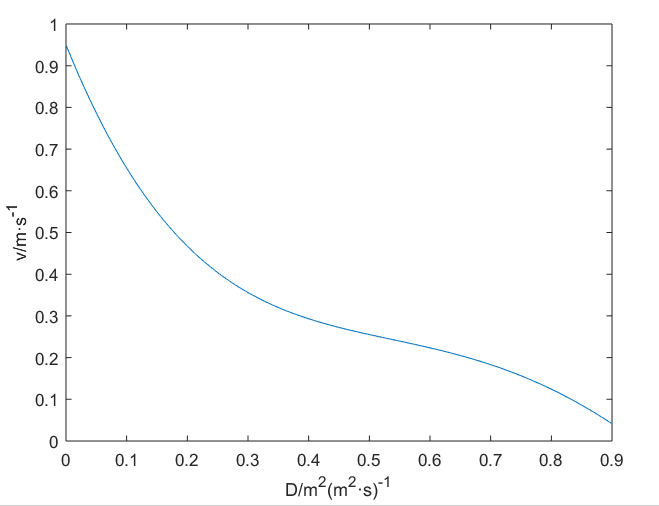
\includegraphics[scale=0.6]{1.png}
    \caption{PF velocity-D diagram}
    \label{1}
\end{figure}
Assuming that the real-time visitor density is $Q_j$ in the jth area and the ending time is $T_j$, we get that
\begin{equation}
    T_j=T_0+\frac{Q_j-\int_0^{T_0}N(t)B\mathrm{d}t}{N^{'}B^{'}}
    \label{equation1}
\end{equation}
where Q represents the number of visitors in the area.

 If there are n exports in the floor, we can get a set of functions $T_j(Q_j),j=1,2,3,...,n$. In order to minimize the total evacuation time, the evacuation time of the exit with the longest evacuation time should be as short as possible. The goal planning function can be expressed as

\begin{equation}
    min\{max\{\{T_j\}\}\},j=1,2,3,...
    \label{equation2}
\end{equation}
   $$ s.t\left\{
    \begin{array}{lr}
    \sum Q_j=Q\\
    0<Q_j<Q\\
    \end{array}
    \right.$$
    
Through the goal programming we can find an optimal solution, and substitute this solution back to (4), we can reverse out a set of ${Q_j}$. By definition, the number of visitors Q in the region is numerically equal to the export capacity F.
%对于一层楼的j个出口,我们可以解出一组$T-Q$的函数关系${T_j{Q_j}}$。要是的总的疏散时间最短,就要是疏散时间最长的出口的疏散时间尽可能的短。

\subsubsection{Available Exit Point Option}

Considering the poor security of other available exits, it is easy to cause security risks. We set a indicator to evaluate whether to use them and the impact of the utilization. We will improve the standard evacuation time calculation formula for public places as a threshold for us to determine whether to use other available exits for evacuation.
%考虑到other available exits的安保情况较差,易导致安全隐患。我们设置了是否使用的指标和使用后的应对方案。我们将改进公共场所标准疏散时间计算公式作为我们判断是否use other available exits进行疏散的阈值,即
\begin{equation}
    t_0=\gamma\{1+\frac{\sum \sum Q_{i,j}}{0.9[A_1(N-1)+A_2Z]}+T_{pass}\}
\end{equation}
\[
\gamma=Ce^{-k}
\]
where $\sum \sum Q_{i,j}$ indicates the number of people in the facility; $A_1$ indicates the capacity of the escalator (unit: $(m·min)^{-1}$); $A_2$ indicates the capacity of the stairs (unit: $(m·min)^{-1}$); $N$ indicates the number of escalators; $Z$ indicates the total width of the stairs; 0.9 indicates that the escalator and stairs are converted by a 10\% discount; $T_{pass}$ represents the time required to reach the exit from the farthest exit of the facility; and $\gamma$ time-risk factor.
%其中,$\sumQ_{i,j}$表示设施内人数;$A_1$表示扶梯的通行能力(单位:$(m·min)^-1$);$A_2$表示楼梯的通行能力(单位:$(m·min)^-1$;$N$表示扶梯数目;$Z$表示楼梯总宽度;0.9表示扶梯和楼梯的通过能力按九折折算;T表示设施内距离出口最远者到达出口所需要的时间;$\gamma$时间-危险系数。

We assume that T represents the actual time required for evacuation.
If T > $t_0$, it means that the four main doors are no longer sufficient for emergency evacuation, and we need to use other available exits. If not, it means that the four main doors have been able to meet the needs of emergency evacuation, and we do not need to use other available outlets.


When other available exits are used, we recommend that the museum take the following measures to ensure that visitors are safely evacuated.

\begin{enumerate}
    \item Add security forces to guide the tourists to evacuate in an orderly manner for the available exits used.
    \item Deliver the information of other available outlets to specific SRZs or several exhibition rooms to prevent widespread dissemination of information, resulting in excessive visitors flocking to the exit
    \item Select other available outlets based on real-time visitor density distribution and regional evacuation efficiency
\end{enumerate}




\section{Real-time Path Planning Model Based on Network}

\subsection{Model Overview and Analysis}

In the above model, we successfully partition the whole floor into several zones and people in the corresponding zones could only walk through the dedicated doors in this zone. Therefore, it is important to consider how to get people from different rooms in this zone to the exit. In this paper, The staircase for this floor is equivalent to the exit for the building. Meanwhile, people on the same floor are notified of emergencies at the same time. When an emergency occurs, people's first reaction is to run to the door of their room or to the narrow corridor connecting the room and the room, where bottlenecks are easily created. In addition, unexpected events such as sudden roof collapsing can increase the risk of roads or create bottlenecks.What we need to do now is to arrange reasonable routes for people, keeping them from bottlenecks and risks.

%在上面的模型中,我们成功地将整个楼层划分成几个区域,相应区域的人只能通过该区域的专用门,因此我们需要考虑如何将该区域不同房间的人带到出口。在本文中,我们认为这一层的楼梯相当于出口。同时,我们认为,同一楼层的人同时收到紧急情况通知。想象一下,在紧急情况下,人们的第一反应是跑向他们房间的门,或者跑向连接房间和房间的狭窄走廊,在那里会由于形成瓶颈。此外,突然的屋顶倒塌等意外情况也会增加道路的风险或形成瓶颈.我们现在要做的就是尽量让被困人员规避这些风险和瓶颈.
 

\subsection{Model Construction}
\subsubsection{The Details about Model}

Any emergency evacuation space can be modeled as $G(v,E)$ network.
To illustrate our model, we take a room with three doors for an example.
%可以将任一的应急疏散空间模化为 G( v, E)网络,为了说明我们的模型我们先以一个拥有三个门的房间作为例子.
%picture
\begin{figure}[ht]
    \centering
    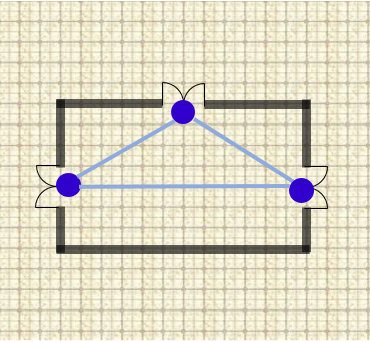
\includegraphics[scale=0.6]{room.png}
    \caption{Network}
    \label{1}
\end{figure}

In the graph, there are three nodes $u_1$,$u_2$,$u_3$, which make up the node set $\{u={u_1, u_2, u_3} \}$ of the space. In the graph, there are three sides, they are $ (u_1, u_2), (u_1, u_3), (u_2, u_3)$. They make up the edge set
$e_i_j=\{(u_i, u_j)\}$ of the space.

We regard the door of each room or the narrow corridor connecting two rooms as nodes. The connection between the two nodes through the exhibition hall is regarded as the edge, so we abstract a concrete terrain into a network.In many emergency response strategies in the past. Visitors always regard the shortest distance to the door as the best escape path,but we think that the shortest distance to reach the exit does not mean the shortest time to reach the exit, since there are many bottlenecks slowing down the speed. Even the path which cost the shortest time to reach the exit can not prove that this is the best path, because the danger coefficient of this road may be very high. People pay the price of damaging their health in order to pass in a shorter time.
%我们将每个房间的门或连接两个房间的狭窄走廊视为节点。两个节点通过展厅的连接被认为是边缘,因此我们将一个具体的地形抽象成一个网络,在过去的许多应急响应策略中,人们总是把到门的最短距离作为最佳的逃生路径,但我们认为到达出口的最短距离并不意味着短距离测试到达出口的时间,因为有许多瓶颈会减慢速度。即使是最短到达出口的路径也不能证明这是最佳路径,因为这条道路的危险系数可能很高。为了在短时间内通过,人们付出了损害健康的代价。

Because danger usually occurs when running from room to room, congestion mainly occurs when queuing at the door.To solve this problem,We set the equivalent length $w_{ij}$ of each edge as
\begin{equation}
  w_i_j=q_i_j\beta_i_j l_i_j
\end{equation}
 %由于危险通常发生在从一个房间跑到另一个房间时,拥挤主要发生在门口排队时。为了解决这个问题,我们将每个边缘的等效长度$w_ij_$
where $q_i_j$ is crowding coefficient of two nodes connected to the edge; $\beta_i_j$ is the danger coefficient of each edge; and $l_{ij}$ is the actual length of this edge.

We define the congestion coefficient as 
\[q_{ij}= \frac{v_{max}^2}{v_iv_j}\]
\[
v=112D^4-389D^3+434D^2-217D+57
\]
where v is a function of the people flow density.
$v_{max}$ is the speed at which people pass through the door when the people flow density is zero.

According to the types of emergencies that occur and the degree of danger that emergencies bring to people in different locations, we give the danger coefficient tto measure the danger degree as
\[\beta_i_j=10^k   \quad k=0,1,2,3,4\]

When a disaster occurs, people's first reaction is to run to the nearest door or follow a familiar person to a random door or look for the door farthest from the disaster., so we use cellular automate (CA) to simulate the initial congestion coefficient of each node in this room
and calculate the the equivalent length of each edge. Each node can choose many routes to reach the final exit. We believe that the path with the shortest sum of the equivalent lengths is the optimal path in this moment.

However, as the crowd starts to flow, the congestion coefficient of nodes and the danger coefficient of edges may change. Therefore, we redesign the route every $\Delta t$ for all those who have not yet arrived at the exit. At this time, many people may not have reached the next node or have left the next node. The number of visitors in an edge is counted into the next node in the network.

\subsubsection{Adaptability of Risk Index k}

According to statistics and information in Knoema and Google, earthquakes, fires, gunpowder terrorist attacks, and biochemical terrorist attacks are the most threatening and frequent disasters or crimes in large venues such as museums.

\paragraph{Earthquake grading M:} Earthquakes are classified into 1-10 levels according to the Ricker series. We assume that people on the same floor have the same risk index and the risk index increases with the floor increases

\paragraph{Classification of fire disaster F :} By considering the area of combustion , the speed of expansion of the fire and the distance from the person to the fire point comprehensively,we can give the risk index.



\paragraph{Classification of gunpowder terrorist attacks T: }This mainly includes gun-type attacks, bomb attacks, and suicide attacks.Calculate the risk index by combining the degree of damage of the attack with the distance of the visitors from the threat

\paragraph{Classification of biochemical terrorist attacks w:} This mainly includes poisonous gas bombs, chemical and biological weapons and other attacks. Based on the data we have investigated, we measure the degree of risk by the concentration of biochemical substances and the speed of transmission.
\[
  w=a\gamma^mv^n  
\]
 among them, a is determined by chemical weapons and properties; $\gamma$ is the ratio of the concentration of biomass to mass; v is the propagation speed of the biochemical liquid-gas substance at the place of use.
 \begin{figure}[H]
    \centering
    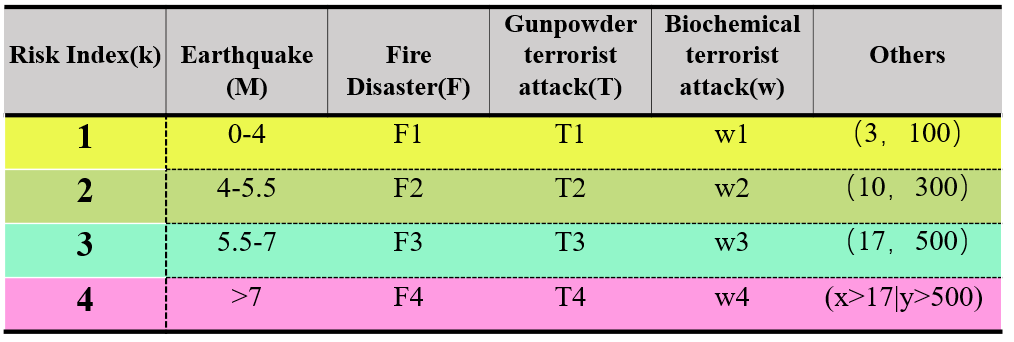
\includegraphics[scale=0.4]{riskindex.png}
    \caption{Risk index}
    \label{1}
\end{figure}
 Here, $(x,y)$ in the column $"Others"$ means, the number of casualties is less than x and the area of the damaged zone is less than y $m^2$.Choose the highest level that can be achieved when defining.

In the event of an emergency security incident, it is difficult for staff to accurately classify disasters. Therefore, we propose a standardized risk grading scheme as Figure 2 to guide staff to respond quickly to threats and select appropriate emergency evacuation plans.

\subsubsection{Calculation of PF in Network Nodes}

If we count the PF of the visitor to the exit, we can know that he obeys a certain distribution. The PF waveform undergoes a series of waveform transformations as it passes through nodes and edges in the network.
%如果对游客到达出口的PF进行统计,我们可以知道他服从一定的分布。PF的波形在通过网络中的一个个节点和边的过程中会进行一系列波形变换。




\begin{itemize}
    \item Time-delaying transform:
\end{itemize}
    The waveform of the PF needs to pass through the nodes and the edge process for a certain period of time, which corresponds to the time required for the flow of people through the exhibition hall and the corridor. This results in the time delaying transform.
    %第四块代码:导入图片
    
    
    \begin{figure}[htbp]
    \centering
    \subfigure{
    \begin{minipage}[t]{0.3\linewidth}
    \centering
    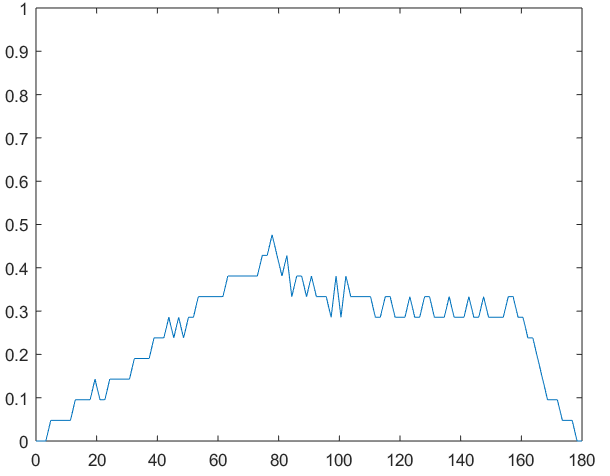
\includegraphics[width=1.8in]{01.png}
    \caption{\\Initial waveform}
    \end{minipage}%
    }%
    \centering
    \subfigure{
    \begin{minipage}[t]{0.3\linewidth}
    \centering
    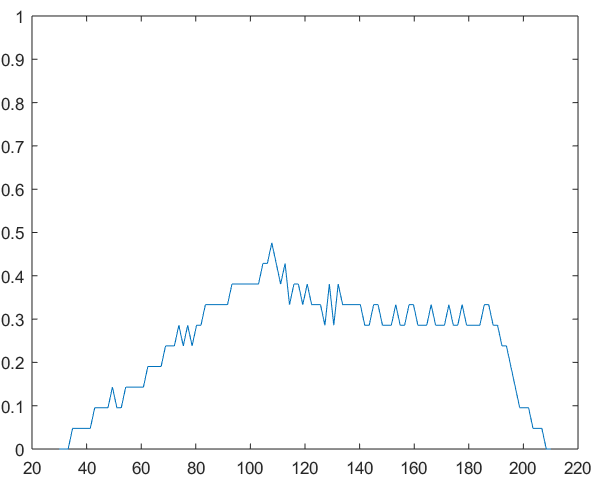
\includegraphics[width=1.8in]{02.png}
    \caption{\\Time-delaying transform}
    \end{minipage}%
    }%
    %\centering
    \subfigure{
    \begin{minipage}[t]{0.3\linewidth}
    \centering
    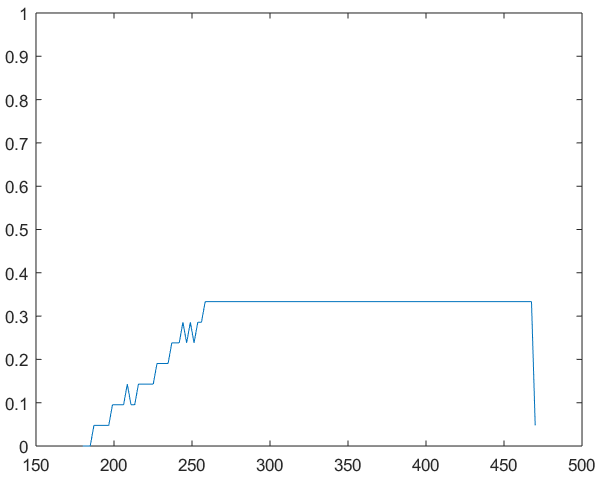
\includegraphics[width=1.8in]{03.png}
    \caption{\\Q-transform}
    \end{minipage}
    }
    \centering
    %\caption{Transforms}
    \end{figure}


    %第四块代码:导入图片

    %PF的波形再通过节点和边过程中都需要通过一定的时间,这对应着人流通过展室和廊道所需要的时间。这导致了时间延迟变换。
\begin{itemize}
    \item Q-transform:
\end{itemize}
When the PF from a wide area to a narrow area, there is a queuing phenomenon here due to the limitation of the channel size. The resulting waveform transform becomes a Queue transform

According to the definition of nodes and edges, we know that nodes are narrow corridors, which are generally prone to Q-transform, while edges are not easy to occur. But the Time-delaying transform is the transformation that takes place on both the nodes and the edges.
%根据节点和边的定义,我们知道节点是较狭窄的廊道,一般容易发生Q-transform,而边则不易发生。但Time-delaying transform 是在节点和边上都要发生的变换。
  %第四块代码:导入图片



\section{Inter-floor Sorting Model}
When people on the higher floor flow to the lower floor, the PF from the upper floor will be pooled with the PF queued here on the lower floor. At this time, the density of tourists will increase rapidly. When the density of tourists exceeds a certain range, it will restrict the movement of individuals and people, and it will easily lead to accidents such as conflicts and trampling. Therefore, we need to analyze the superimposed PF waveform and guide the staff to guide the way and time of the two PFs to be collected.
%当高层的人流向低层流动时,从楼上下来的PF会和低层在这里排队的PF发生汇集现象。这时,游客密度会迅速增大,当游客密度超过一定范围后,会限制个人和人群移动,而且极易引发冲突和踩踏等事故。因此,我们需要通过对他们superimposed PF waveform进行分析,指导工作人员引导两股PF会汇集的方式和时间。

Here, we introduce the relationship between population density and population behavior in previous studies to guide us in solving this problem.
%这里,我们引入前人的研究的人群密度和人群行为的关系,来指导我们解决这一问题。
%第五块代码:绘制表格
\begin{table}[H]
\centering
\begin{tabular}{c|c}
\toprule
Crowd density&Group condition\\
\midrule
5&People can contact with each other's clothing\\
\midrule
6&People can pick up items and turn around\\
\midrule
7&People's shoulders and elbows will have a sense of squeeze\\
\midrule
8&A person can barely pass between two people\\
\midrule
9&People's behavior is limited, their hands can't move up and down,\\ &creating a sense of anxiety\\
\midrule
10&People feel a lot of pressure from the surroundings, the body can't move,\\ &there is a cry for help, and it is easy to have a stampede accident.\\
\bottomrule
\end{tabular}
\caption{The relationship between population density and population behavior}
\end{table}

We can see that when the density exceeds $7m^{-2}$, the crowd is prone to accidents. Therefore, the staff should prevent the density of visitors at the stairway and at any queue point from exceeding $7m^{-2}$.
%我们可以看到当密度超过$7m^{-2}$时,人群中极易发生事故。因此工作人员要防止在楼梯口处和任意一个排队点的游客密度超过$7m^{-2}$。

%我们通过下面的例子,来展示我们前面的PF计算对层间人流汇聚的指导意义。
The following examples are used to demonstrate the guiding significance of our previous PF calculations for the convergence of people between floors.
Through the Time-delaying transform and Q-transform mentioned above, we can calculate the waveform of any node in the network that flows to the exit or stairway. When any two streams meet, they will be superimposed to form a new waveform.
%通过上文提到的Time-delaying transform和Q-transform 我们可以计算出网络中任意一个节点的人流传到出口处或楼梯口处的波形,当任意两股人流相遇时会叠加形成新的波形。


From the example, the result of the superposition is less than 0.7, and the corresponding tourist density is less than $7m^{-2}$. Therefore, at this gathering point, there is no need for staff to drain visitors. But we must be vigilant and guide people to maintain order.
%从算例中看,两者叠加的结果小于0.7,对应的游客密度小于 $7m^{-2}$。因此,在这个汇聚点,不需要工作人员对游客进行引流。但必须提高警惕,引导人们保持秩序。
When the situation turns into a PF upstairs and a PF pool that is being queued downstairs, the waveform is superimposed as
%当情况变成楼上的PF和楼下正在排队的PF汇集时,波形叠加为
\begin{figure}[H]
    \centering
    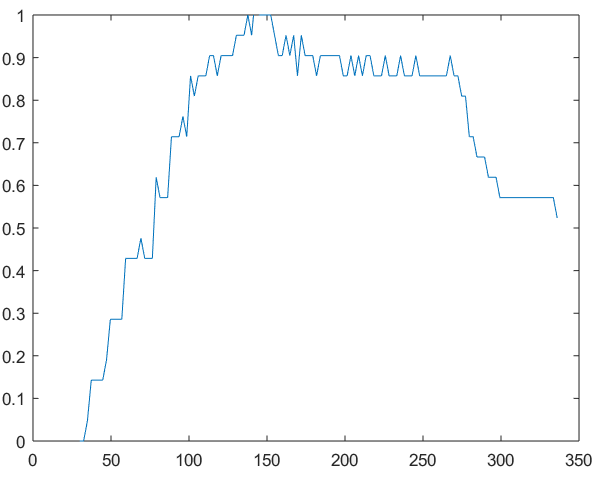
\includegraphics[scale=0.6]{06.png}
    \caption{Superimposed inter-floor PF waveform }
    \label{1}
\end{figure}

From the example, the result of the superposition is more than the corresponding tourist density is greater than $10m^{-2}$. Therefore, at this stairway, the staff upstairs should guide some tourists to evacuate to other stairways in advance or ask the upstairs tourists to wait for a while, keep order, and inform the staff downstairs to evacuate the tourists as soon as possible.
%从算例中看,两者叠加的结果超过了,对应的游客密度大于 $10m^{-2}$。因此,在这个楼梯口,楼上的工作人员要提前疏导部分游客到其他楼梯口疏散或者要求楼上游客暂时等待一下,保持秩序,并通知楼下工作人员尽快疏散游客。

\section{Model Solution and Analysis}
\subsection{Forecast of the Number of Tourists}
%我们假设卢浮宫的疏散情况发生在2019年,所以首先对2019年的疏散情况进行预测。在2007-2018年卢浮宫游览人数基础上,我们发现一年内游览卢浮宫的总人数总体较为稳定,并呈现出较小的周期性变化。所以,我们用傅里叶曲线拟合,预测得到2019年卢浮宫的游客数为$10658792$人。

We assume that the evacuation of the Louvre occurred in 2019, when we need to forecast the number of visitors. Based on the number of visitors to the Louvre in 2007-2018, the Fourier curve fitting is utilized to predict that the number of visitors to the Louvre in 2019 will be \textbf{$10,658,792$}.

%为了更精确地对卢浮宫的疏散情况进行计算,我们需要得到卢浮宫的游客人数数据。鉴于无法直接得到卢浮宫的日访客人数变化表,所以我们基于一些规则通过计算机模拟计算出了卢浮宫的日访客人数。

In order to calculate the evacuation of the Louvre more accurately, we need to get data of the specific number of visitors to the Louvre. We calculated the number of visitors to the Louvre by computer simulation based on some rules.


%日访客人数与开放时间正相关。卢浮宫一周内开放时间不同,会造成日访客人数的周期性变化。
%总体人数变化服从正态分布。
%周二会有残障访客参观,不计入模型考量范围内。全年残障访客$2100$人,相较于数百万的普通游客数太小。
%举办展览时游客数增加。据了解,卢浮宫有春展和秋展,还会举办免费夜场,这些时间段游客数增加。
%假期时间段游客数量增加。
%学生的长假期间游客数增加较多。资料显示,$51%$的卢浮宫游客在30岁以下。也就是说,很多卢浮宫的游客都是学生。所以我们认为长假时间段游客数量增加。
%不同国家游客的假期时间段可能不同。美国、中国游客数多,所以我们认为美国、中国假期期间卢浮宫游客数增加明显。


The rules are as follows:
\begin{itemize}
    \item The number of visitors per day is positively related to the opening hours. The opening hours of the Louvre in a week will cause periodic changes in the number of visitors per day.
    \item There will be disabled visitors on Tuesday, which are not counting the model considerations. There are $2100$ of disabled visitors throughout the year, which is too small compared to millions of regular visitors.
    \item The number of visitors increased during the exhibition. It is understood that the Louvre has a spring exhibition and autumn exhibition, and will also host a free night market. The number of visitors increased during these time periods.
    \item The number of tourists increased during the holiday period.
\end{itemize}

%卢浮宫一年内开放3215.2小时。结合我们预测的2019年游客人数和以上规则,我们认为:2019年内卢浮宫一天内最少访客数为$21345$人,最多访客数为$52660$人,平均每天访客数为$52660$人

The Louvre opened $3215.2$ hours a year. Combined with our forecast of the number of visitors in 2019 and the above rules, we calculate that the minimum number of visitors per day in the Louvre is \textbf{$21,345$} in 2019, with a maximum of \textbf{$526,60$} and an average of \textbf{$526,60$} per day.

\subsection{Calculation of Emergency Evacuation Time}
Based on the daily visiting data for the Louvre's annual statistics, we select data for visitors to a certain day in July 2019. A random simulation of the distribution of visitor density on the Louvre day at each floor.The reason why we randomly simulate the distribution of tourists is because we cannot get specific data. But we know that the daily data of the Louvre every day varies greatly and does not have regularity, while the Louvre generally has a large flow of people in the pyramid gate, Mona Li Sasha and Broken Arm Venus. We meet these conditions during our simulation. Therefore, the simulation we have made is also realistic to some extent.
%我们根据依据对卢浮宫年度统计的日客流量数据,选取2015年7月某日参观游客的数据。对卢浮宫当天的游客密度在每一层的分布进行随机模拟。我们需要指出的是选择随机模拟游客的密度分布与相关数据难以获取有关,但我们知道卢浮宫每年每天的游客数据变化很大,不具有规律性,同时卢浮宫一般在金字塔、蒙娜丽莎和断臂维纳斯等处的人流量较大,我们在模拟时满足了这些情况。因此我们所做的模拟也是在一定程度上符合实际的。
We first select the situation of the day and briefly explain the operation process.It is assumed that there was a fire on the first floor of the venue at 13:14 pm this day and there are 927 visitors here. Through computer simulation, we get the distribution image after the flow of people go through the stairs.
%我们首先选取当天一层的情况简单说明运算过程。我们假设这一天下午13:14分在场馆内第一层发生了大火。通过计算机模拟我们得到了,人流到达楼梯口时的分布图像。
\begin{figure}[H]
    \centering
    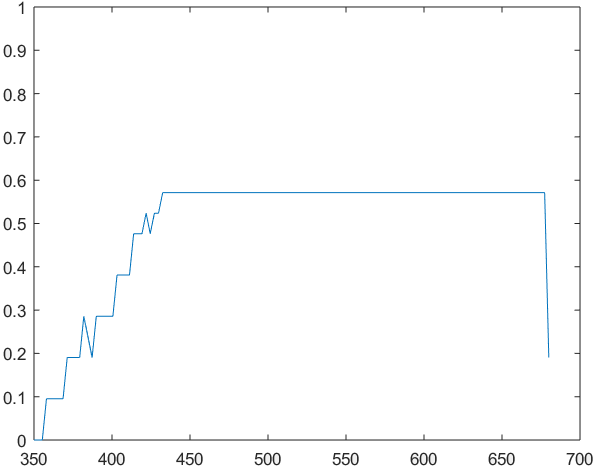
\includegraphics[scale=0.6]{04.png}
    \caption{Superimposed PF waveform at a stairway}
    \label{1}
\end{figure}

We can get an approximate expression for this image.
%我们可以得到这个图像的近似表达式。
    $$D(t)\left\{
    \begin{array}{lr}
    4.59\times10^{-3}t-1.6065,350<t<480\\
    0.597,480<t<678\\
    \end{array}
    \right.$$
    
Through the measurement we calculated that the average width of the six stairs or escalators on this floor is 2.8m. At the same time, the average width of our visitors is 0.5m. The projected channel flow density threshold can be calculated as $\eta=0.367$.
%通过测量我们计算出,该层六个楼梯或扶梯的平均宽度为2.8m。同时,我们取游客的平均宽度为0.5m。可以计算出投影化的通道人流密度阈值为$\eta=0.367$。

When the visitor passes through the stairway, $D(t)$ is Q-transformed.
%当游客从楼梯口通过后,$D(t)$进行了Q-transform。
    $$D^*(t)\left\{
    \begin{array}{lr}
    4.59\times10^{-3}t-1.6065,350<t<429.96\\
    0.597,429.96<t<631.11\\
    \end{array}
    \right.$$
    
When we substitute this function $D^*(t)$ and parameters into equation \ref{equation1} and \ref{equation2}, we can use MATLAB to solve the target function $min\{max\{\{T_j\}\}\}, j=1, 2, 3,...$.
%当我们将这一函数$D^*(t$和参数代入$(4)$$(5)$中,我们可以利用MATLAB求解目标函数$min\{max\{\{T_j\}\}\},j=1,2,3,...$。
\[
T_1=T_2=T_3=T_4=T_5=T_6=459s
\]
\[
\{Q_j\}=\{100.8016,173.4728,156.6091,155.4747,198.4536,141,4097\}
\]

It indicates the optimal time for evacuation in the 1st floor is 8min7s. We substitute the calculated data into (1) to calculate a set of regional radius values.
%我们把计算数据代入(1),可以算出一组区域半径值。
\[
\{R_j\}=\{198.12,101.73,167.84,123.76,134.60,179.22\}
\]

We give the partition mode of this floor according to the partition radius as shown in the figure below.
%我们根据分区半径给出这一层的分区模式如下图所示。
\begin{figure}[H]
    \centering
    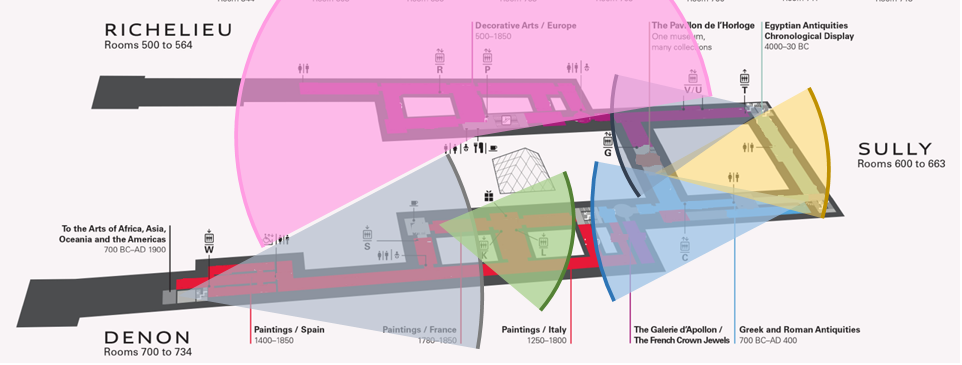
\includegraphics[scale=0.3]{huafen.png}
    \caption{SRZ Division Diagram}
    \label{1}
\end{figure}


Based on the time-shifted results of the simulated PF waveform, we learned that the group of people reached the lower floor through the stairs for 187 seconds in the 1st SRZ. Using the intra-floor planning method above, we can calculate the time to exit from the stairway to the doorway is 207s.
%根据模拟的PF波形的时移结果,我们得知这群人通过楼梯到达下方楼层的时间为187s。利用上文中的层内规划方法,我们可以计算出从楼梯口到达门口离开的时间为207s。(以上)

\begin{figure}[H]
    \centering
    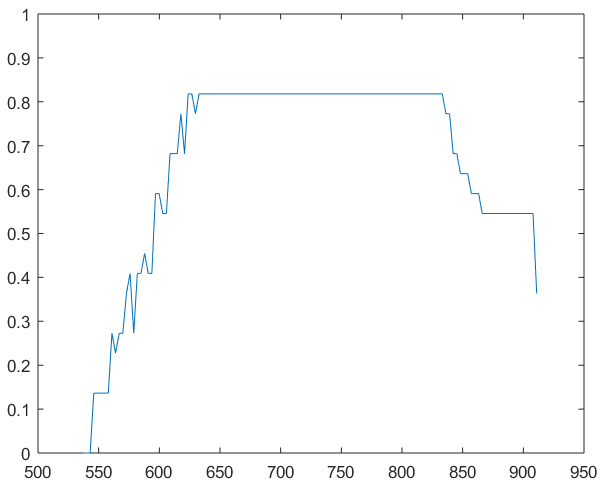
\includegraphics[scale=0.37]{05.png}
    \caption{PF Waveform after the Stairway}
    \label{1}
\end{figure}

Therefore, we can calculate the total evacuation time of all partitions of the five floors as ${t_{i,j}}$, which indicates the evacuation time of the $ith$ floor $jth$ SRZ. We know that the final evacuation time can be expressed as $max\{t_{i,j}\}$. In this example, we calculated the total evacuation time $t=16min46s$.In this example, we calculated the total evacuation time $t=16min46s$.
%于是,我们可以计算五层楼所有分区的的疏散总时间为{t_{i,j}},这表示ith层jth SRZ 的疏散时间。我们知道最终的疏散时间可以表示为$max\{t_{i,j}\}$。在这一例子中,我们计算出的疏散总时间$t=16min46s$.

\subsection{Optimal Path Selection}

We assume that the fire occurred on the edge between node and node 2, but the disaster is not very serious. Therefore, we set the hazard index here to be $k=2$. According to the initial parameters we set for each of our floors, we can calculate by formula $(7)$ that the equivalent coefficients of different nodes and edges are
\[
\{[\omega_j];[\epsilon_j]\}=\{[5.4,689.71,7.8,6.6,4.3,7.8,6.8,9.1];[78.34,
24.31,27,88,87.91,88.34,54.66,54.36]\}
\]
%我们假设火灾发生在节点1,2之间的edge上,但灾情并不是很严重。因此,我们设置这里的危险指数为k=2。依据我们我们每一层设置的初始参数我们可以计算出,不同节点和边的当量系数为

\begin{figure}[ht]
    \centering
    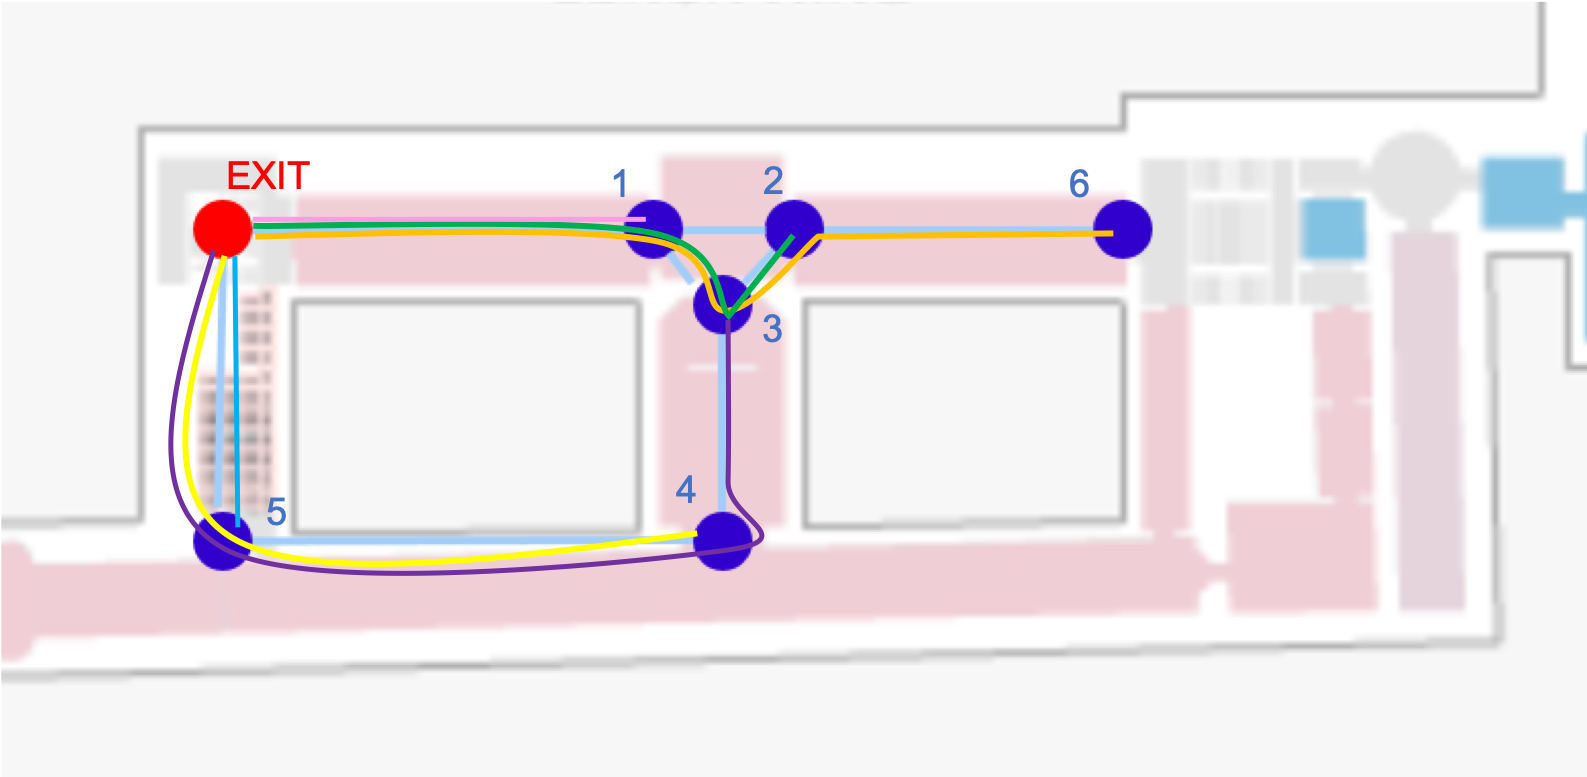
\includegraphics[scale=0.4]{han9.png}
    \caption{Optimal Path Selection in a SRZ}
    \label{1}
\end{figure}

The figure above is a demonstration of our optimal path for an SRZ calculation. In the same way, our model can guide different SRZ staff to guide visitors on different nodes to choose the optimal path for their escape.
%上图是我们对一个SRZ计算的最优路径的展示。用同样的方法我们的模型可以指导不同SRZ工作人员指导不同节点上的游客选择适合他们逃生的最优路径。






\section{Priorization Scheme}

\subsection{Overview and Analysis}
In the previous paper, we have established a general emergency evacuation model, but we still have many problems to consider, such as the appropriate time that the emergency personnel should enter the building, the best route for disabled people to escape and the way for people from different countries to know the emergencies more effectively . To solve these problems, we give reasonable suggestions through our analysis.
% 在前文我们建立了大致的人员疏散模型,但我们仍然有许多问题需要考虑比如应急人员该何时进入建筑,残疾人该如何逃生,来自不同国家的人如何较为有效的知道紧急情况的发生等等,对于这些问题,我们通过分析给出合理的建议。
\subsection{Emergency Personnel Entry Plan}
It is vital that emergency personnel should enter the building at first. By consulting the literature, we know that the highest turntable ladder is 101 meters. Therefore, when an emergency occurs in the high building , emergency personnel can first take the ladder to enter or take helicopter to reach the floor where disaster occur. Although some emergency personnel can arrive quickly, most of them still have to enter the building through the door.  we designed adaptable entry schemes according to the total number of people in the building.

Taking the Louvre as an example, we design an entry plan fore mergency personnel .

When the density of visitors in the building is less than $5m^{-2}$. At this time, we can use the Richelieu entrance for the evacuation of tourists on the first and the second floors. Personnel can evacuate some tourists on the the floor who is far away from the Richelieu entrance and those on the negative floor from the exit on the two negative floor. The Portes Des Lions entrance without the evacuation of tourists is used as the entrance for emergency personnel.

When the density of tourists is greater than $5m^{-2}$ but less than $8m^{-2}$, we think that all the main doors should be used to evacuate tourists. Emergency personnel can enter the special access by the main door for them.

When the density of tourists is greater than $8m^{-2}$, we think that the density of tourists is beyond the load range of the main door. At this time, we will open available exit for emergency personnel to enter and other available doors for visitors to evacuate.
%第四块代码:导入图片
\begin{figure}[ht]
    \centering
    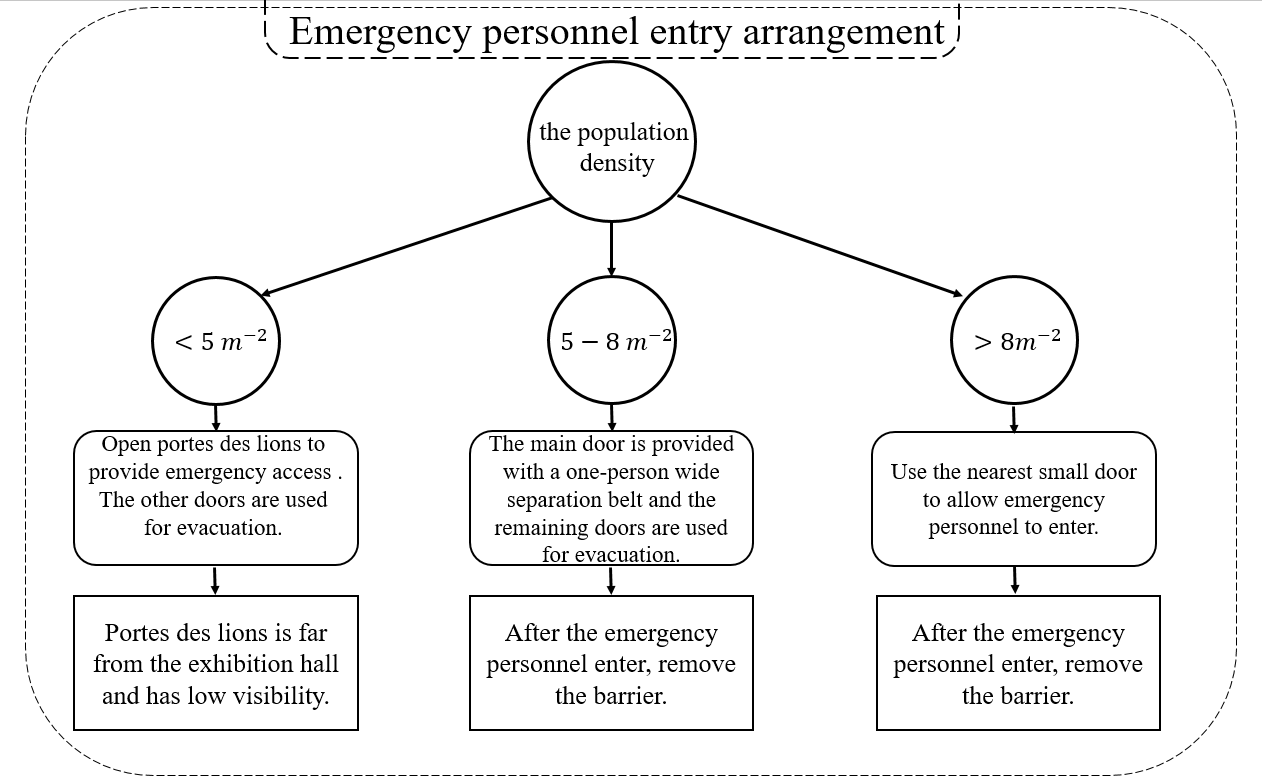
\includegraphics[scale=0.3]{sun.png}
    \caption{Emergency Personnel Entry Plan}
    \label{1}
\end{figure}







 %一个热门景点的人流量每年和每天都在变化,但是我们认为无论何时应急人员都应该率先进入。通过查阅资料我们得知最高的云梯为101米,相当于四十多层楼的高度,因此当紧急情况发生在高层的时候,应急人员可以先乘坐云梯进入或者乘坐直升机到达灾难发生的楼层。虽然一些急救人员可以很快到达,但他们中的大多数人仍然必须通过门进入大楼。
 
 %以卢浮宫为例,我们设计了正常到达应急人员的进入方案,当建筑中的游客密度小于。。。。,这时我们可以将黎塞留门用于一楼和二楼游客的疏散,将0层远离门口的部分游客和-1层的游客从-2层的出口疏散了,没有游客疏散的师门作为应急人员的进入门
 %当游客密度大于什么什么小于什么什么的时候我们认为所有的主要的门都应该用来疏散游客,应急人员可以从在主要的四个门的旁边为他们专门开辟的通道进入
 %当人流密度很大的时候,我们认为除了所有主要的门要用于疏散游客之外,一些只有工作人员知道的小门也要开始使用。将其中一个离事故发生点最近的小门作为应急人员的进入通道,在应急人员进入一段时间后再开放这个门让游客使用

\subsection{Visitor Characteristics Analysis and Solutions}

\begin{itemize}
    \item \textbf{Tourists' linguistic diversity}
\end{itemize}

By reading the information, we can learn that the main languages used by visitors to the Louvre include: French, English, German, Italian and Chinese. The multilingual nature of visitors can hinder the delivery of evacuation orders during emergency evacuation. In response to this problem, let us give some measures to optimize our evacuation plan.
 %查阅资料,我们可以获知参观卢浮宫的游客所使用的主要语言包括:法语、英语、德语、意大利语和汉语等。游客的多语言特性会在紧急疏散对疏散指令的传达形成阻碍。针对这一问题,我么给出一下措施优化我们的疏散方案。
 
 \begin{enumerate}
     \item During the emergency evacuation, the staff use the broadcasting equipment in the venue to conduct French-British bilingual command evacuation.
     %紧急疏散时,工作人员利用场馆内广播设备进行法英双语指挥疏散。
     \item  The museum should strengthen foreign language training for staff in densely populated areas and important venues, where staff and security personnel with foreign language skills are resident.
     %加强对人员密集区域和重要场馆的工作人员的外语培训,在这类区域常驻具有外语能力的工作人员和安保人员。
     \item In the case of emergency evacuation, evacuate instructions in multiple languages are sent on the application.
     %紧急疏散时,在应用程序上发送多种语言的疏散指令。
     \item The Louvre will provide simultaneous interpretation on the app.
     %在应用程序上提供同声传译功能。
 \end{enumerate}

\begin{itemize}
    \item \textbf{Tourist group problem}
\end{itemize}

According to statistics, more than 60\% of tourists visited the Louvre in units of two or more. In the case of emergency evacuation, visitors tend to act together emotionally and behaviorally, which can cause some problems for our evacuation, especially when the group is very large. But if the museum chooses not to allow all groups that violate the evacuation order to act together, it is also very unfriendly. In fact, it is a reasonable emergency evacuation plan to allow a group to be dismantled within an acceptable range. Here we have the following standards.
%从统计数据上来看,超过60\%的游客是以两人以上的单位进入卢浮宫参观的。在紧急疏散时,通行游客在情感上和行为上都倾向于一起行动,这会对我们的疏散造成一些困扰,尤其是在这个团体很大的时候。但是如果博物馆选择不允许所有有违疏散指令的团体一起行动,也十分不和人情。事实上,在可以接受的范围内,允许一部分团体不被拆散才是合理的紧急疏散方案。这里我们制定了以下标准。
 \[
 \Delta=\chi\frac{n \Deta t}{N}
 \]
where $\Delta$ denotes the acceptable group number; N denotes the number of booths; $\chi$ denotes the convergence coefficient; t denotes the difference between the evacuation threshold and the actual theoretical evacuation time.
 %这里$\Delta$表示趋同容许值;N表示展室数目;$\chi$表示趋同系数;t表示疏散阈值和实际理论疏散时间的差值。
 
 \begin{itemize}
    \item \textbf{Evacuation of disabled tourists}
\end{itemize}
 
The disabled are required to take special care of the staff during emergency evacuation. At the same time, if the disabled and the normal person are evacuated together, they are both vulnerable and hinder the actions of the crowd. Therefore, when our staff finds disabled people, we need to arrange someone to lead them to transfer from the staff passage or the elevator.
 %残疾人在紧急疏散时由于生理上的缺陷,需要工作人员的特殊关照。同时,如果残疾人和正常人一起疏散既容易受到伤害,又会阻碍人群的行动。因此,我们的工作人员在发现残疾人时,要安排专人带领他们从员工通道或直梯转移。
 
\subsection{Crowd Management and Control Procedure}

In the event of a public safety incident, visitors will exhibit the following behavioral characteristics due to fear, panic and herd mentality:
%在公共安全事件发生时,受恐惧、惊慌和从众心理的影响,游客会表现出如下行为特征:
\begin{itemize}
\item \textbf{Preemptive behavior for passing} visitors will show up in the various passages and push and push, so that they can leave as soon as possible.
%游客会在各类通道口表现出插队、推搡行为,以使自己尽快地离开。
\item \textbf{Inertial behavior} The evacuating staff often fall into the inertia trap when evacuating, and the visitors are impressed by the familiar entrances and exits, which leads to crowds.
%进行疏散的工作人员在进行疏散时常常会陷入惯性陷阱,将游客印象自己熟悉的出入口,从而导致人群拥堵。
\item \textbf{Dodge behavior} people have the nature of being profitable and avoiding harm. When a hazard occurs, people prefer to travel around the road rather than passing through the danger.
%人具有趋利避害的本性。当危害发生时,人宁愿绕远路,也不愿从危险发生处通行。
\end{itemize}

Therefore, it is very important to strengthen the emergency evacuation training for staff and to convey correct and timely instructions. This requires us to reasonably arrange the location of the staff and the number of staff in different locations during evacuation. It can be proved that important venues, access intersections and stairways as well as exits are locations where accidents are likely to occur. We set $\omega_1(\rho,n)$, $\omega_2(d,B,p)$,$\omega_3(\rho,n)$, measuring the importance of a location by three weighting indicators. We calculate the number of staff in this SRZ by calculating the sum of the weight values within an SRZ. At the same time, we have to arrange more staff in the large location of $\omega$ in SRZ, especially those with foreign language ability and security personnel.
%因此,加强对工作人员的应急疏散培训和传达正确的及时的指令只会游客转移都十分的重要。这要求我们要在疏散时合理的安排工作人员的位置和不同位置上工作人员的多少。我们认为重要场馆、通道交汇处和楼梯口以及出口是事故易发生的位置。我们设置$\omega_1(\rho,n)$,$\omega_2(d,B,p)$,$\omega_3(\rho,n)$,三个权重指标来衡量。我们以计算一个SRZ内的权重值之和来安排这个SRZ内工作人员数量。同时我们要在SRZ内$\omega$很大的位置安排更多的工作人员,尤其是由外语能力的人员和安保人员。





\section{Sensitivity Analysis}

We have conducted a sensitivity analysis of the Safety Response Zone Division Model.

%考虑到模型较大,且较为复杂,所以我们用精确度并不高的元胞自动机对二楼进行仿真。我们改变模型中一个展厅的长度和宽度参数,并观察对结果的影响。
Considering that the model is large and complex, a cellular automaton with low accuracy is used to take simulation. Therefore, we use a cellular automaton with low accuracy to simulate the second floor. The length and width parameters of an exhibition hall is changed in the model, and then we observe the effect on the results.

    \begin{figure}[H]
    \centering
    \subfigure{
    \begin{minipage}[t]{0.3\linewidth}
    \centering
    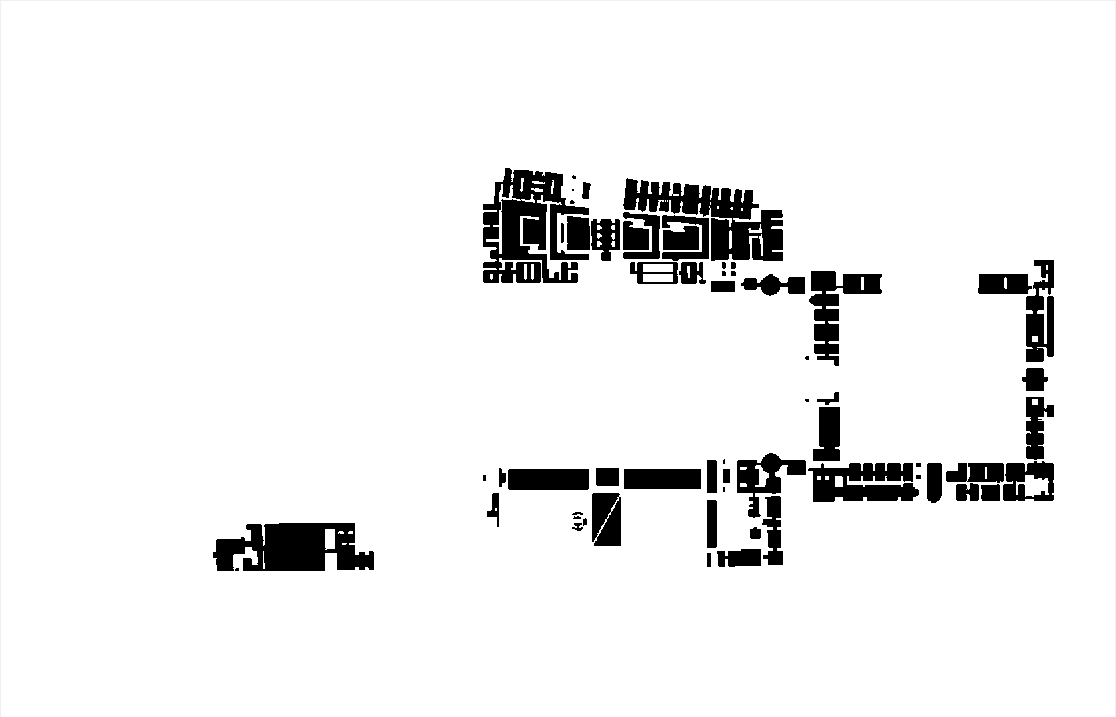
\includegraphics[width=1.8in]{21.png}
    \caption{\\Background}
    \end{minipage}%
    }%
    \centering
    \subfigure{
    \begin{minipage}[t]{0.3\linewidth}
    \centering
    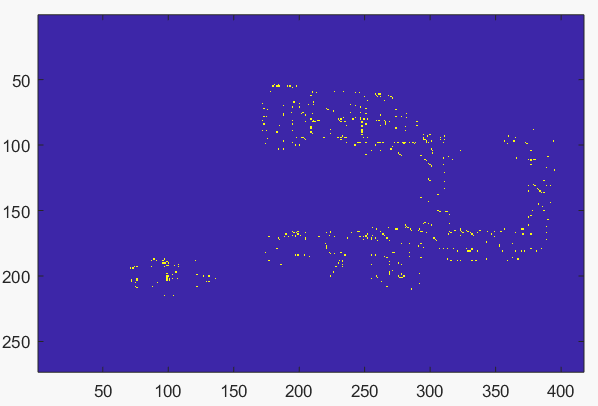
\includegraphics[width=1.8in]{32.png}
    \caption{\\Cellular automaton}
    \end{minipage}%
    }%
    \centering
    \end{figure}

%从图像上我们可以看到在一层楼的范围内元胞自动机的行动过程图。我们保证其它条件一致(人数等),调整其中一间展厅的长度和宽度参数。考虑到元胞的运动情况有一定的随机性,所以我们经过多次仿真并得到平均值,结果如下表:

\begin{table}[!htbp]
\centering
\begin{tabular}{|c|c|c|}
\hline
\multicolumn{3}{|c|}{One Exhibition Hall}\\ % 用\multicolumn{3}表示横向合并三列 
                        % |c|表示居中并且单元格两侧添加竖线 最后是文本
\hline
Length&Width&Average Evacuation Time\\
\hline
15& 10& 459s\\
\hline
10& 10& 463s\\
\hline
\end{tabular}
\caption{Evacuation time change}
\end{table}

%我们看到,一间展厅距离缩短后,疏散时间增加了。我们认为原因有两个:
We notice that the evacuation time increased after the distance between one exhibition hall is shortened. We reckon there are two reasons:

%元胞自动机行为的随机性。其随机性来自于我们对游客初始位置设置的随机性。
%展厅长度变短后,撤离游客数增加。这导致总的撤离时间边长。

\begin{itemize}
    \item The randomness of cellular automata behavior. Its randomness comes from our randomness in setting the initial position of the visitor.
    \item After the length of the exhibition hall became shorter, the number of evacuated visitors increased. This results in a total evacuation time.
\end{itemize}

%总体来看,两次仿真的时间相差不大,这表明我们模型的结果在参数微小改变后变化不大。我们的模型是可靠的。
Overall, the time between the two simulations is not much different, which indicates that the results of our model do not change much after a small change in parameters. Our model is reliable.

\section{Strengths and Weaknesses}
\subsection{Strengths}
    \paragraph{Quantified and rational goals} We set quantified goals strictly based on optimal path planning theory
    \paragraph{Robustness and flexibility} The fundamental strength of our model comes from its enormous flexibility,where most of the parameters in our model is not fixed. Furthermore, our model has the notion of time,which is omitted in most mathematical model.
    \paragraph{Easy to understand} adopting a hierarchical structure, our model can be easily understood with single graph and several pictures of explanation.

%  我们的模型具有很强的适应性,可以根据不同的紧急情况设定不同的逃生路线
%  我们的模型具有低复杂性,我们将层与层之间的人流移动量化的表示了出来,并为每个出口划定了辐射范围,这样有效的缩短了撤离时间。
%  我们的模型具有很高的完成度,对于可能影响卢浮宫紧急疏散的各种因素都给出了详细的解释。

\subsection{Weaknesses}
    \paragraph{Potential invalid assumptions}Another obstacles that may hold back our model's performance is that the assumptions made to simplify the model may be invalid,therefore leading to a less useful model.
    \paragraph{Potential vulnerability due to the lack of data} The fundamental weakness of our model also comes from data. Since we can't obtain the accurate data of the Louvre, there is a lot of uncertainty in the validation of our model.
    \paragraph{}
%由于许多数据难以收集,因此模型只能进行一部分的验证。
%对于一些地图中难以分辨的楼梯,我们选择了忽略它们的存在。
%对于一些没办法具体量化的问题,我们只是给出了解决方案。



\newpage

\bibliography{yinyong}

\newpage

\begin{appendices}
\section{Appendix: Data}

    \begin{table}[ht]
    \centering
    \begin{tabular}{c|cccccc}
    \toprule
    Year&2013&2014&2015&2016&2017&2018\\
    \midrule
    Number of tourists&$9.3$million&$9.3$million&$8.6$million&$7.4$million&$8.1$million&$10.2$million\\
    \bottomrule
    \end{tabular}
    \caption{Number of yearly visitors to the Louvre.}
    \end{table}
    
\section{Appendix: Code}
      
\subsection{Picture Conversion}      
\lstset{language=Matlab}
        
\begin{lstlisting}
    close all;
    clear;clc;
    %%
    %Image reading and conversion (reading, grayscale, filtering effective space, removing noise, reducing image)
    %Image reading
    floor0 = imread('floor0.png');
    %subplot(3,2,1),imshow(floor0);
    %grayscale
    gfloor0 = rgb2gray(floor0);
    figure(1),imshow(gfloor0);%Effective color center value:221 226 178 215 237
    gfloor0(gfloor0(:,:)>=217&gfloor0(:,:)<=225) = 0;
    gfloor0(gfloor0(:,:)>=222&gfloor0(:,:)<=230) = 0;
    gfloor0(gfloor0(:,:)>=174&gfloor0(:,:)<=182) = 0;
    gfloor0(gfloor0(:,:)>=211&gfloor0(:,:)<=219) = 0;
    gfloor0(gfloor0(:,:)>=233&gfloor0(:,:)<=241) = 0;
    gfloor0(gfloor0(:,:)~=0) = 255;
    len = size(gfloor0,1);
    wid = size(gfloor0,2);
    %figure(1),imshow(gfloor0);
    for j = 1:20
        for i = 1:len
            for j = 1:wid
                if gfloor0(i,j)<=5
                    mat = gfloor0(i-2:i+2,j-2:j+2);
                    num = sum(mat(:)==0);
                    if num <= 9
                        gfloor0(i,j) = 255;
                    end        
                end
            end
        end
    end 
    %figure(1),imshow(gfloor0);
    len = size(gfloor0,1);
    wid = size(gfloor0,2);
    for i = 1:len/4
        nfloor0(i,:) = gfloor0(4*i-1,:);
    end
    for i = 1:wid/4
        mfloor0(:,i) = nfloor0(:,4*i-1);
    end
    %imshow(mfloor0);
    pfloor0 = double(mfloor0); 
    figure(2),imagesc(pfloor0);
\end{lstlisting}

\subsection{Estimated Number of Visitors Per Day}      
\lstset{language=Matlab}
        
\begin{lstlisting}
    %Estimated number of visitors per day.
    mon = normrnd(28088,2000,52,1);
    tue = normrnd(40,10,52,1);
    wed = normrnd(43712,2000,52,1);
    thu = normrnd(28088,2000,52,1);
    fri = normrnd(43712,2000,52,1);
    sat = normrnd(28088,2000,52,1);
    sun = normrnd(28088,2000,52,1);
    years = [mon,tue,wed,thu,fri,sat,sun];
    yearr = [reshape(years',1,364),normrnd(28088,3000,1,1)];
    %china
    yearr(181:240) = yearr(181:240)+300;
    yearr(1:60) = yearr(1:60)+300;
    %us
    yearr(151:240) = yearr(151:240)+700;
    yearr(335:365) = yearr(335:365)+700;
    %show
    yearr(1:210) = yearr(1:210)+500;
    yearr(300:365) = yearr(300:365)+500;
    plot([1:365],yearr)
    %with Tuesday
    big = max(max(yearr))
    smalltue = min(min(yearr))
    %without
    sm = min(years);
    sm(:,2) = [];
    small = min(min(sm))
\end{lstlisting}
      
  \end{appendices}


